\documentclass[a4paper,12pt]{report}

\usepackage[utf8]{inputenc}
\usepackage[T1]{fontenc}
\usepackage[french]{babel}
\usepackage[top=20mm, bottom=25mm, left=15mm, right=15mm]{geometry}
\usepackage{hyperref}
\usepackage{mathpazo}

\usepackage{graphicx}
\usepackage{pgfplots}

\usepackage{amsmath}
\usepackage{amssymb}
\usepackage{mathrsfs}

\usepackage{fancyhdr}

\setlength{\parindent}{3em}
\setlength{\parskip}{1em}

\setcounter{secnumdepth}{3}
\renewcommand{\thesection}{\arabic{section}}
\renewcommand{\thesubsection}{\arabic{section}.\arabic{subsection}}
%\titleformat{\subsubsection}[runin]{\normalfont\bfseries}{\thesubsubsection}{0em}{}

\pagestyle{fancy}
\fancyhead[L]{Projet GE2}
\fancyhead[C]{\textit{Aéroglisseur radiocommandé}}
\fancyhead[R]{Étude - Avril 2020}
\fancyfoot[L]{INSA Strasbourg}
\fancyfoot[R]{Tristan DRUSSEL - Florian POUTHIER}
\headheight=14.5pt

\title{Rapport d'Étude Projet GE II\\Aéroglisseur radiocommandé}
\author{Tristan DRUSSEL - Florian POUTHIER \\ \\ Génie Électrique 4ème année\\ INSA Strasbourg}
\date{Année scolaire 2019-2020}

\begin{document}
	\begin{titlepage}
		\maketitle
	\end{titlepage}
	\tableofcontents
	\newpage
	
	\section{Introduction}
	
	Dans le cadre de notre formation Génie Électrique à l'INSA Strasbourg, le \textbf{projet GE II} du semestre 8 a pour objectif la conception d'un système électrique comprenant des éléments de conversion statique et de commande électronique programmable. Ce projet sera notamment l'occasion de mettre en œuvre nos connaissances acquises en électronique de puissance, en électronique numérique, en informatique industrielle et en automatique tout au long de notre cursus. 
	
	Le thème retenu cette année consiste en une compétition baptisée "La nuit de la glisse". L'objectif sera de présenter pour cette compétition un \textbf{aéroglisseur radiocommandé} qui devra répondre à un certain nombre d'exigences pour pouvoir être homologué et ainsi participer à l'épreuve finale. En vue de réaliser un tel système, nous partirons d'un cahier des charges succinct pour mener une analyse fonctionnelle du dispositif, rédiger un cahier des charges complet et finalement concevoir, simuler, tester et fabriquer l'aéroglisseur attendu.
	
	Ce projet sera également pour nous l'occasion de développer nos compétences linguistiques dans la langue anglaise par le biais de rapports oraux ponctuels lors des différentes étapes de développement du système. Les aspects linguistiques ciblés sont notamment la maîtrise du vocabulaire technique relatif au thème du projet ainsi que la maîtrise de formes classiques comme les formes passives. Nous serons également amenés à travailler avec des documents techniques et des ressources bibliographiques en langue anglaise tout au long du projet.
	
	Le projet intégrera finalement les aspects humains de gestion de projet et de communication orale et écrite. Nous ferons vérifier dans un premier temps nos lettres de motivation et CV, pour ensuite définir une stratégie de projet basée autour d'un planning de travail. Les présentations orales de pré-étude, de définition de solution, d'étude... seront réalisées en salle banalisée et filmées afin d'obtenir un meilleur débriefing sur nos méthodes de communication et sur l'amélioration de celles-ci.
	
	\newpage
	
		\section{Moteur brushless DC de propulsion}
		
		\vspace{-1em}
		
		Le \textbf{moteur DC brushless} (en anglais \textit{Brushless DC Motor}, abrégé BLDCM par la suite) est un moteur qui a connu un gain en popularité très important au cours des deux dernières décennies. Et pour cause, les champs d'application de ce type de moteur sont multiples : appareils électroménagers, automobile, aérospatial, équipement médical, production industrielle et instrumentation \cite{AN885}. 
			
		Le moteur \textbf{NM Prodrive 3350 110kV} retenu pour la conception de notre aéroglisseur est un moteur DC brushless. Il sera notamment utilisé dans notre système pour la rotation de l'hélice, qui permettra à la fois la propulsion et la génération du flux d'air nécessaire à la création du coussin d'air qui supportera l'aéroglisseur.
			
			Dans cette partie, nous développerons dans un premier temps les généralités autour des moteurs DC brushless. Dans un second et troisième temps, nous aborderons les aspects de conception d'un onduleur et de contrôle du moteur avec une méthode ne faisant appel à aucun capteur basée sur la lecture du retour de force électromécanique. Une quatrième partie se concentrera sur les aspects de réalisation d'un PCB de contrôle 
			
			\vspace{-1em}
		
			\subsection{Généralités}
			
			\vspace{-1em}
			
			Comme son nom l'indique, et contrairement à la majorité des moteurs DC, le BLDCM n'utilise pas de balais pour sa commutation. La commutation est au contraire réalisée électroniquement. L'utilisation de cette structure fait que le BLDCM a de nombreux avantages par rapport aux moteurs DC à balais ou les moteurs à induction. Parmi ces avantages, on peut notamment retenir :
			
			\vspace{-1em}
			
			\begin{itemize}
				\item[$\bullet$] un meilleur compromis couple / vitesse 
				\item[$\bullet$] un temps de réponse amélioré
				\item[$\bullet$] une durée de vie prolongée
				\item[$\bullet$] un fonctionnement moins bruyant
				\item[$\bullet$] des rangs de vitesse plus élevés
			\end{itemize}
			
			De plus, le rapport couple délivré / encombrement moteur est amélioré, ce qui rend le BLDCM très utile dans des applications où l'espace et le poids sont des critères cruciaux \cite{AN885}, comme dans le cas de notre aéroglisseur.
			
			\vspace{-1em}
			
				\subsubsection{Structure du BLDCM}
				
				\vspace{-1.5em}
				
				 Un moteur brushless est structuré à partir d'un aimant permanent au rotor et de pôles bobinés au stator. L'énergie électrique est convertie en énergie mécanique par le biais des forces d'attraction magnétique entre l'aimant permanent du rotor et le champ tournant induit par les pôles bobinés du stator. La \textsc{Figure \ref{struct_bldcm}} présente une illustration simplifiée de la construction d'un BLDCM. 
				 
				 \begin{figure}
				 	\begin{center}
				 		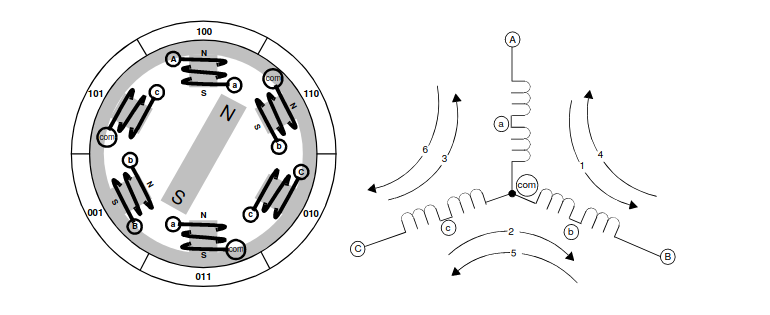
\includegraphics[scale=0.7]{../Illus/struct_bldcm.png}
				 	\end{center}
				 	\caption{Diagramme simplifié de la structure d'un BLDCM (\textit{Source :} \cite{AN857})}
				 	\label{struct_bldcm}
				 \end{figure}
				 
				 L'exemple de structure présenté ici montre trois circuits électomagnétiques connectés à un point commun (couplage étoile). Chacun des circuits est divisé en deux parties qui seront bobinées sur des dents de la machine diamétralement opposées. Cette structure permet alors à l'aimant permanent au rotor de se déplacer au milieu de champs magnétiques induits. Nous avons modélisé le BLDCM en utilisant le logiciel \textit{FEMM} pour donner une idée plus concrète de son fonctionnement en rotation. La montre notamment la modélisation de la structure du moteur sur ce logiciel.
				 
				 % Capture d'écran structure FEMM électif circuit magnétique

				 La plupart des BLDCM ont une structure triphasée avec un couplage étoile, et c'est notamment le cas du moteur que nous allons utiliser dans ce projet. Un tel moteur est alors piloté en alimentant deux phases en même temps. Afin d'entrer en rotation, les trois phases du moteur devront être alimentées 
				 
				 \subsubsection{Séquence de commutation}
				 
				  % Récupérer modélisation FEMM de l'électif circuits magnétiques S4
				  
				 \subsubsection{Structure d'un onduleur triphasé}
				 
				 \subsubsection{Modélisation électrique du BLDCM}
				 
				 \subsection{Conception de l'onduleur triphasé}
				 
				 \subsection{Méthode de contrôle du BLDCM}
				 
				 Le BLDCM que nous avons retenu pour 
				 
				 	\subsubsection{t}
				 
				 
				 
				 
				 
				 
				 
				 
				 

			
			\subsection{Contrôle basé sur le retour de force électromotrice}
	
		\chapter{Interface d'alimentation}
		
		Afin de fonctionner dans son intégralité, le système a besoin de différents niveaux de tension, parmi lesquels un niveau de 5V pour le servomoteur et l'alimentation des microcontrôleurs, et du 3.3V pour l'utilisation du \textit{Bluetooth Low Energy}. Il est donc prévu de concevoir à cet effet un PCB permettant d'obtenir tous les niveaux de tension nécessaires sur une seule carte et ainsi les distribuer à tous les éléments fonctionnels du système.
		
			\section{Caractérisation de la source d'alimentation}
			
			La source d'alimentation de notre projet est une \textbf{batterie LiPo 3S}. Ce type de batterie est structuré par 3 cellules LiPo de 3.7V en série, soit une \textbf{tension nominale de 11.1V} (3 x 3.7V) pour la batterie LiPo 3S à vide. Un élément LiPo est en fait une batterie Li-ion où l'électrolyte est un polymère gélifié.
			
			Il est à garder en mémoire que la décharge d'un élément LiPo en-dessous de 2.5V entraîne sa destruction. De manière générale, il est recommandé de ne pas décharger les éléments en-dessous de 3.3V si l'on souhaite une durée de vie optimale pour ce type de batterie. 
			
		A l'inverse, chaque élément LiPo \textbf{ne doit jamais être chargé au-dessus de 4.2V}, au risque de provoquer un \textbf{possible incendie}. Dans le cas d'une batterie constituée d'éléments LiPo multiples, il est \textbf{impératif d'utiliser un \textit{égaliseur}} dans le circuit de charge.
		
		% Source : http://geeby22.over-blog.com/page-4287873.html
			
			\section{Conversion tension batterie vers 5V}
			
			L'alimentation des microcontrôleurs et du servomoteur nécessite d'obtenir un niveau de tension de 5V à partir de la tension 11.1V de la batterie LiPo 3S. Pour cela, nous avons mis en oeuvre le régulateur à découpage \textbf{LM22672MR-5.0/NOPB} du constructeur \textit{Texas Instruments}. Ce régulateur permet d'implémenter un convertisseur de type Buck en utilisant un minimum de composants externes. Toutefois, ces derniers devront être correctement dimensionnés afin de prendre en compte les contraintes de la source et de la charge.
			
			\subsection{Généralités sur le composant LM22672}
			
				\subsubsection{Caractéristiques électriques}
			
				\subsubsection{Schéma d'application standard}
				
				La Figure \ref{schema}
			
			\subsection{Dimensionnement du convertisseur}
			
				\subsubsection{Données }
				
				\subsubsection{Dimensionnement des composants}
				
					\paragraph{Diode Schottky}
					
					La diode Schottky de sortie retenue pour le montage est la \textbf{SL22-E3/52T} du constructeur \textit{Vishay}. Elle est notamment adaptée à des applications de convertisseurs DC/DC comme le montage que celui que nous souhaitons dimensionner. La \textsc{Table \ref{charact_schottky}} \cite{SL22}.
					
					\begin{table}
						\begin{center}
							\begin{tabular}{|l|c|c|c}
							\hline
							Paramètre & Symbole & Valeur & Unité \\
							\hline						
							Tension maximale inverse & $V_{RRM}$ & 20 & V \\
							\hline						
							Tension maximale efficace & $V_{RMS}$ & 14 & V \\
							\hline						
							Courant maximal direct & $I_{F}$ & 2.0 & A \\
							\hline						
							\end{tabular}					
						\end{center}
						\caption{}
						\label{charact_schottky}
					\end{table}
				
					\paragraph{Condensateurs d'entrée}
					
					Comme dans tout dimensionnement de convertisseur, une attention particulière doit être portée au choix des condensateurs d'entrée du montage. Leur but principal est notamment de \textbf{réduire l'ondulation sur l'entrée du convertisseur}. Une bonne pratique est de choisir des \textbf{condensateurs céramiques} ayant des \textbf{valeurs d'ESR très faible} afin de réaliser cette fonction. Ils doivent notamment être placés au plus proche de l'entrée du convertisseur pour obtenir le meilleur effet possible \cite{A055}.
								
						\subparagraph{Paramètres influents le dimensionnement}
						Les différents paramètres intervenant dans le dimensionnement des condensateurs d'entrée du montage sont en particulier :
						
						\begin{itemize}
							\item[$\bullet$] le courant $I_{S}$ nominal dans la charge ;
							\item[$\bullet$] le rapport cyclique  $\alpha_{nom}$ au point nominal de fonctionnement ;
							\item[$\bullet$] la fréquence $F$ de commutation du convertisseur.	
						\end{itemize}
						
						La relation (\ref{c_in_th}) permet de déterminer pratiquement la valeur minimale de la capacité à placer en entrée en considérant tous les paramètres énoncés ci-dessus.
						\begin{equation}
							C_{min} = \frac{I_S\cdot\alpha\cdot(1-\alpha)\cdot 1000}{F\cdot V_P}
							\label{c_in_th}
						\end{equation}
						
						\subparagraph{Calcul de la capacité d'entrée nécessaire}
						
						En vue d'appliquer la relation (\ref{c_in_th}), on prendra les valeurs d'application numérique suivantes :		
						\begin{equation}
							F = 575.061\text{kHz} 
							\quad\text{;}\quad
							\alpha = 0.44201
							\quad\text{;}\quad
							I_S = 1\text{A}
						\end{equation}
						
						\subparagraph{Pertes dans les condensateurs d'entrée}
						
						Les pertes dans les condensateurs suivent la relation de Joule :
						
						\begin{equation}
							P = R \cdot I^2
						\end{equation}
						
						où R est la valeur de l'ESR de
						
								
							\paragraph{Condensateurs de sortie}
							
							Tout comme les condensateurs d'entrée, les condensateurs de sortie d'un convertisseur font l'objet d'un dimensionnement particulier. Cependant leur rôle est tout autre : ils doivent, en association avec l'inductance de sortie \cite{A055}.	
				
				
			
			\subsubsection{Ajustement de la fréquence de commutation}
			
			Le composant LM22672 est capable de fonctionner 
			
			\subsection{Simulation du convertisseur}
			
			Le dimensionnement précédent
			
				\subsubsection{Modélisation du convertisseur sous \textit{LTSpice}}
				
				\subsubsection{Essais de charge}
				
				\begin{figure}[h]
\begin{center}
\begin{tikzpicture}
\begin{axis}[
	x=500cm,
	y=0.9mm,
	axis x line=middle,
	axis y line=middle,
	xmin = 0, xmax = 0.001,
	ymin = 0, ymax=20,
	grid=both,
	xlabel=Temps (s),
	ylabel=$V_{OUT}$ (V)
]

\addplot[color=blue]
table[x expr=\thisrowno{0}*1000,y={V(v_out)}]
{data/load_transient.txt};

\addplot[color=orange]
table[x={time},y={I(I1)}]
{data/load_transient.txt};

\end{axis}
\end{tikzpicture}
\end{center}
\label{filtre_th}
\caption{Diagramme de Bode en module de la fonction de transfert théorique $H_{Th}(p)$}
\end{figure}
				
				\subsubsection{•}
				
			
			\subsection{Dimensionnement thermique}
			
			Tous les montages électroniques qui contiennent des semi-conducteurs, condensateurs ou d'autres composants vulnérables à l'action thermique vont avoir une durée de vie largement limitée si on ne prend pas en compte les aspects thermiques lors du dimensionnement. Aussi vital soit-il pour améliorer , le dimensionnement thermique est rarement facile 	
			
			La puissance dissipée par le convertisseur, $P_D$, peut être déterminée facilement.
			
			\begin{equation}
				P_D = V_{OUT}\cdot I_{OUT}\cdot\left(\frac{1}{\eta}-1\right)
			\end{equation}	
			
			\begin{equation}
				P_D  = 5V\cdot
			\end{equation}							
			
			% AN-2020 TI
			
			
			\subsection{Routage du convertisseur}
			
				\subsubsection{Synthèse des composants}
				
				La \textsc{Table \ref{synth_composants}} résume l'ensemble des composants à intégrer au PCB pour réaliser le convertisseur 12V vers 5V. Elle précise notamment les références des sites \textit{RS} et \textit{Farnell} afin de faciliter l'étape de commande de composants. Sont aussi répertoriés les boîtiers des composants afin de préparer toutes les empreintes nécessaires à la réalisation du PCB.
				
				\begin{table}
					\begin{center}
						\begin{tabular}{|c|c|c|c|c|}
						\hline
						\textbf{Ref Schéma} & Ref. \textit{RS} & Ref. \textit{Farnell} & Ref Fabricant & Boîtier \\ 
						\hline
						C\_BOOT & 461-4013 & & C0805KRX7R9BB103 & 0805 \\
						\hline
						C\_IN & 434-8126 & & C0805KRX7R9BB103 & 0805 \\
						\hline
						C\_IN2 & 451-5770 & & C0805KRX7R9BB103 & 0805 \\
						\hline
						C\_OUT & 795-5691 & & C0805KRX7R9BB103 & 0805 \\
						\hline
						C\_SS & 698-3425 & & C0805KRX7R9BB103 & 0805 \\
						\hline
						D\_1 & 184-1516 & & C0805KRX7R9BB103 & 0805 \\
						\hline
						L\_1 & 813-5684 & & C0805KRX7R9BB103 & 0805 \\
						\hline
						LM22672 & 761-5450 & & C0805KRX7R9BB103 & 0805 \\
						\hline
						RT & 123-3056 & & C0805KRX7R9BB103 & 0805 \\
						\hline
						\end{tabular}
					\end{center}
					\caption{Synthèse des composants du convertisseur 12V vers 5V sur le PCB d'alimentation}
					\label{synth_composants}
				\end{table}
				
				
				
				
				
			
		\section{Conversion 5V vers 3.3V}
			
		Le composant \textbf{MCP1826S-3302E/EB} de \textit{Microchip} a été retenu pour établir la conversion 5V vers 3.3V. Ce régulateur linéaire fournissant une sortie faible tension et un courant de 1000mA typique a été choisi dans sa version sortie standard fixe 3.3V. Le composant est stable en utilisant en sortie un condensateur céramique de valeur 1uF, ce qui facilite largement son dimensionnement. Seulement une capacité d'entrée sera à déterminer pour mettre en œuvre le régulateur.
	
		\subsection{Contrôle de la direction}
			L'aéroglisseur doit pouvoir tourner dans toutes les directions pour pouvoir traverser le parcours. La direction s'effectue en orientant la dérive de l'aéroglisseur, celle ci orientera le flux d'air et ainsi induira un mouvement de rotation à l'ensemble du système. L'actionneur que nous avons pour réaliser le déplacement de la dérive est un servomoteur.
			\subsubsection{Servomoteur}
			Un servomoteur est un moteur asservi en position ou en vitesse. Grâce à un signal de commande caractérisé plus loin, le moteur rejoint une position angulaire ou une vitesse donnée. L'emploi de ce type d'actionneur est simple, une alimentation fixe en 0-5V et un signal de commande permet la réalisation simple de système contrôlé angulairement. Le mot "servo" ne vient pas de cerveau qui signifierait intelligent mais du latin \textit{servus} qui signifie esclave. Il s'agit donc d'un moteur esclave, plus précisément un moteur asservi.
			
			Le signal de commande employé pour contrôlé les servomoteurs est un signal de type PWM (Power Width Modulation, Modulation à Largeur d'Impulsion). La largeur de l'impulsion correspond à une position donnée. Le signal est un signal électrique de période 20ms, toutes les 20ms, le moteur doit recevoir un signal de commande pour s'aligner correctement. La largeur de l'impulsion varie généralement entre 0.5 et 3ms. La largeur d'impulsion fait varier proportionnellement l'angle de sortie ou la vitesse. Par exemple, si une impulsion de 0.75ms correspond à un angle de $0^{\circ}$ et une impulsion de 2.25 à un angle de $180^{\circ}$. Pour obtenir un angle de $66^{\circ}$, il faut une impulsion de 1.3ms.   
			\subsubsection{Génération du signal}
			Afin de générer le signal de commande pour le servomoteur, nous allons utiliser le \textbf{PIC16F1619}. Ce composant programmable nous permettra de générer le signal comportant une impulsion de largeur variable toutes les 20ms. Pour cela, on utilisera un signal PWM de fréquence adaptée, en jouant sur le rapport cyclique, nous jouons sur la largeur de l'impulsion. Cette largeur d'impulsion sera contrôlée par les information transmise sur la liaison \textit{bluetooth}. En effet, en fonction des contrôles demandé par 
		\subsection{Interface de radiocommande}
			Afin de contrôler la vitesse, la direction et potentiellement d'autres aspects de l'aéroglisseur, nous devons établir une communication entre l'utilisateur et le système. La technologie utilisée dans ce projet est la technologie Bluetooth. Cette technologie a commencé à se déployer en 1998, mais elle a explosé dans les années 2010 avec l'apparition massive des appareils nécessitant une communication à faible distance. Depuis de plus en plus d'appareils utilisent cette technologie qui ne cesse de s'améliorer avec l'apparition par exemple du Low Energy.
			\subsubsection{Module Bluetooth}
			Le module Bluetooth que nous utilisons est le module HC-05. Ce module permet d'établir une connexion bluetooth avec un autre appareil. Il communique ensuite en USART avec le microcontrôleur.
			\subsubsection{Application smartphone}
	
	\section{Conclusion}
	
	Ce rapport de pré-étude a pour objectif de présenter le thème du projet GE II ainsi que les objectifs à atteindre en vue de proposer un système fonctionnel et homologable pour la compétition finale en fin de semestre. Nous y exposons une analyse fonctionnelle du système à réaliser, un cahier des charges détaillé ainsi qu'un développement des sous-fonctions du dispositif à concevoir.
	
	La conception d'un aéroglisseur radiocommandé est un projet d'envergure faisant appel à des notions d'électronique de puissance comme d'électronique numérique. Chaque membre du binôme ayant un attrait plus important pour l'une des deux matières, nous avons décidé de nous répartir la charge de travail par domaine de connaissances. Un des membres du binôme développera alors la partie liée à la communication Bluetooth, [...] tandis que l'autre membre du binôme se concentrera sur la commande du moteur Brushless DC ainsi que la génération des différents niveaux de tension nécessaires au fonctionnement du dispositif.
	
	Ce rapport de pré-étude va ainsi nous donner une solide base d'investigation pour le développement de solutions technologiques fiables et fonctionnelles dans la conception de notre système. Afin d'avoir un meilleur suivi de notre avancée, vous trouverez notre répertoire \href{https://github.com/tristanplouz/ProjetGE2}{github ici}.
	
	\listoffigures
	
	\bibliographystyle{plain} 
	\bibliography{biblio.bib}
	
\end{document}
